\section{Systemarkitektur}
\label{chap:systemarkitektur}

Efter at have udarbejdet kravspecifikation, systemskitse og domain model, var der formet en ide om hvordan systemet skulle fungere. I det følgende beskrives hvordan systemarkitekturen er udformet. 

Systemarkitekturen er udført ved brug af SysML og UML diagrammer. 
SysML bruges til beskrivelse af systemets hardware i blokke og som samlet system. Ud fra N + 1 og applikations modellen udformes UML diagrammer, der bruges til beskrivelse af systemets software. 
Foruden SysML og UML diagrammer benyttes en række andre diagrammer, i det følgende beskrives nogle af mest centrale diagrammer.\\


\textbf{Use case}\\
Use cases og tilhørende diagrammer er benyttet i projektforløbets indledende faser. De bruges til at definere systemets kunnen og opdele systemet i mindre dele. Use cases har i høj grad fungeret som et omdrejningspunkt, hvorfra alt funktionalitet udspringer.

\textbf{Domainmodel}\\
Domain modellen er brugt som en overgang mellem kravspecifikation og systemarkitektur.
I kravspecifikation beskrives hvad der sker ved interaktion med systemet. Mens
systemarkitekturen bruges til at beskrive systemet i blokke og til at skitsere både interne
og eksterne forbindelser. Domain modellen bruges til at beskrive hele systemets domæne.
Der kigges ikke på hardware vs. software, der kigges i stedet på "enheder"og deres
ansvarsområder.

\textbf{SysML}\\
Der er benyttet to slags SysML diagrammer til dokumentation af systemets hardware. Block definition diagrammer (bdd'er) er brugt til at identificere og beskrive systemets hardware blokke og deres indbyrdes forhold. Internal block diagrammer (ibd'er) er brugt til at vise de identificerede blokkes interne og eksterne forbindelse, hvordan blokkene kommunikere og hvilke signaler der flyder imellem dem.


\textbf{UML}\\
På baggrund af use cases og domain modellen laves pakkediagrammer, der bruges til at beskrive ansvarsområder i systemet. Sekvensdiagrammer bruges til at identificere systemets klasser, klassernes metoder samt timing i systemet. Klasser samt tilhørende metoder og attributter beskrives ved hjælp af klassediagrammer. State machines bruges til at beskrive flow mellem forskellige states. 


\newpage
 
\subsection{Blokbeskrivelser}
Det overordnede bdd på figur \ref{fig:bdd_asd} viser hvilke hardware blokke systemet består af, samt hvilke parts blokkene indeholder.

\begin{figure}[H]
	\centering
	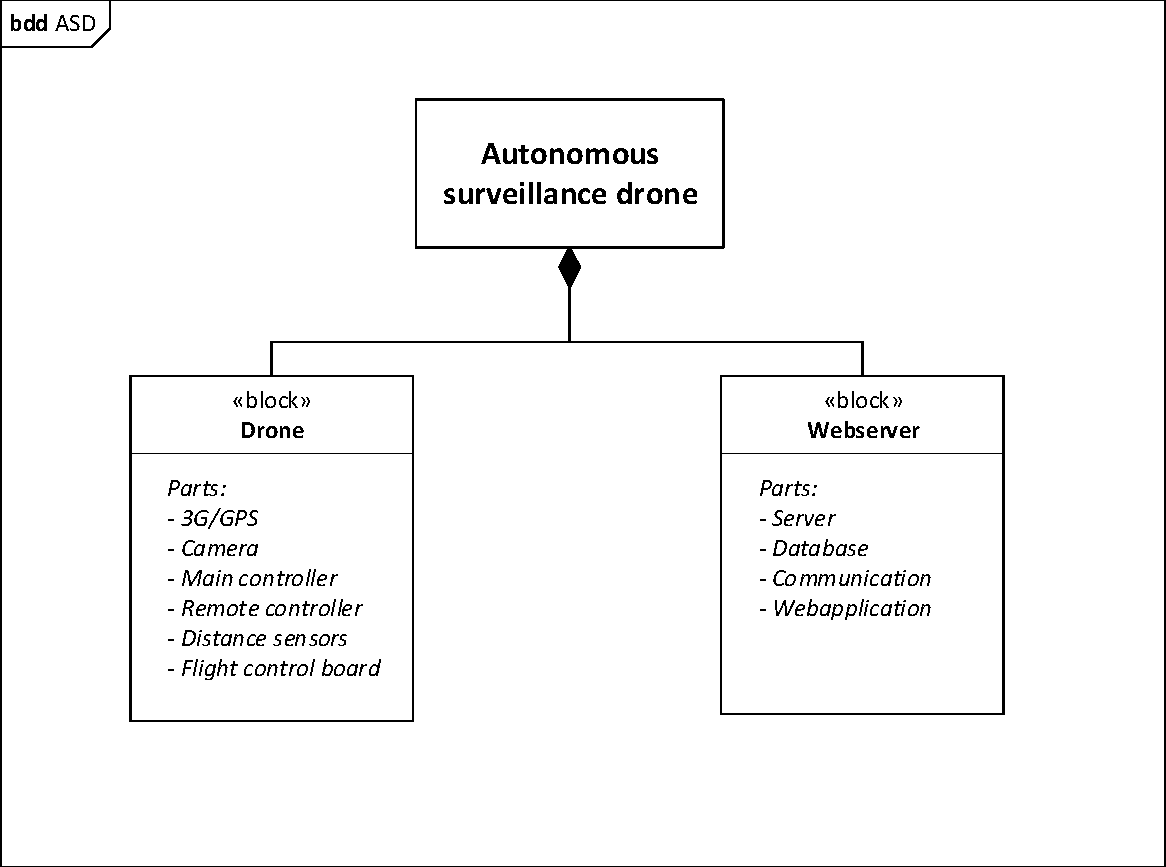
\includegraphics[width=1.0\textwidth]{Billeder/Projektbeskrivelse/bdd_overordnet.pdf}
	\caption{Overordnet bdd for systemet}
	\label{fig:bdd_asd}
\end{figure}

\textbf{Drone} \\
Drone blokken indeholder alt funktionalitet tilhørende drone. De interne forbindelse mellem de forskellige parts er beskrevet i bdd'er som findes i \textit{Systemarkitektur og Design} [X].

\textbf{Webserver} \\
Webserver blokken indeholder server, database, communication og webapplikationen.

\newpage

\subsection{Interne forbindelser}
\vspace{-0.3cm}	
Det overordnede ibd for systemet vises på figur \ref{fig:ibd_asd}. Dels beskriver ibd'et hvordan  systemets største blokke kommunikerer med hinanden og omverden. Desuden beskriver ibd'et hvilken type signaler der anvendes mellem blokke og omverden. 

\begin{figure}[H]
	\centering
	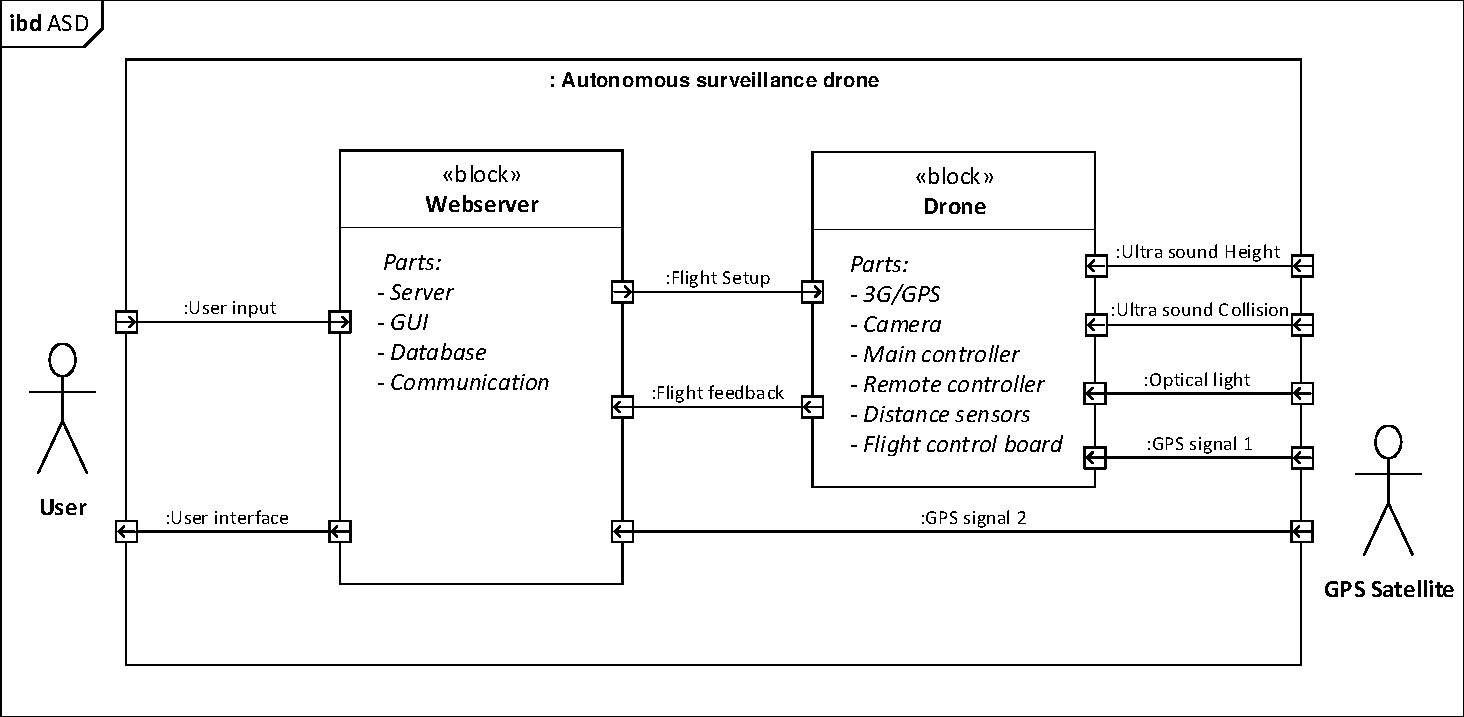
\includegraphics[width=1\textwidth]{Billeder/Projektbeskrivelse/ibd1_overordnet.pdf}
	\caption{Overordnet ibd for systemet}
	\label{fig:ibd_asd}
\end{figure}

Der vises ikke udvidede ibd'er for webserver, da webserver ikke indeholder hardware og derfor beskrives nærmere ved brug af UML diagrammer i software afsnittet. For en beskrivelse af alle udarbejdede ibd'er til drone henvises til dokumentationens \textit{Systemarkitektur og Design} [X].

\subsection{Pakke diagram}
\vspace{-0.3cm}	
Pakkediagrammer bruges i software design afsnittet til at vise hvilke ansvarsområder hver pakke har. På figur \ref{fig:package_drone} ses de overordnede pakker tilhørende dronen. Pakkerne og deres ansvarsområde bruges til at danne grundlag for udformning af softwareklasser og klassernes indbyrdes forhold.
 
\begin{figure}[H]
	\centering
	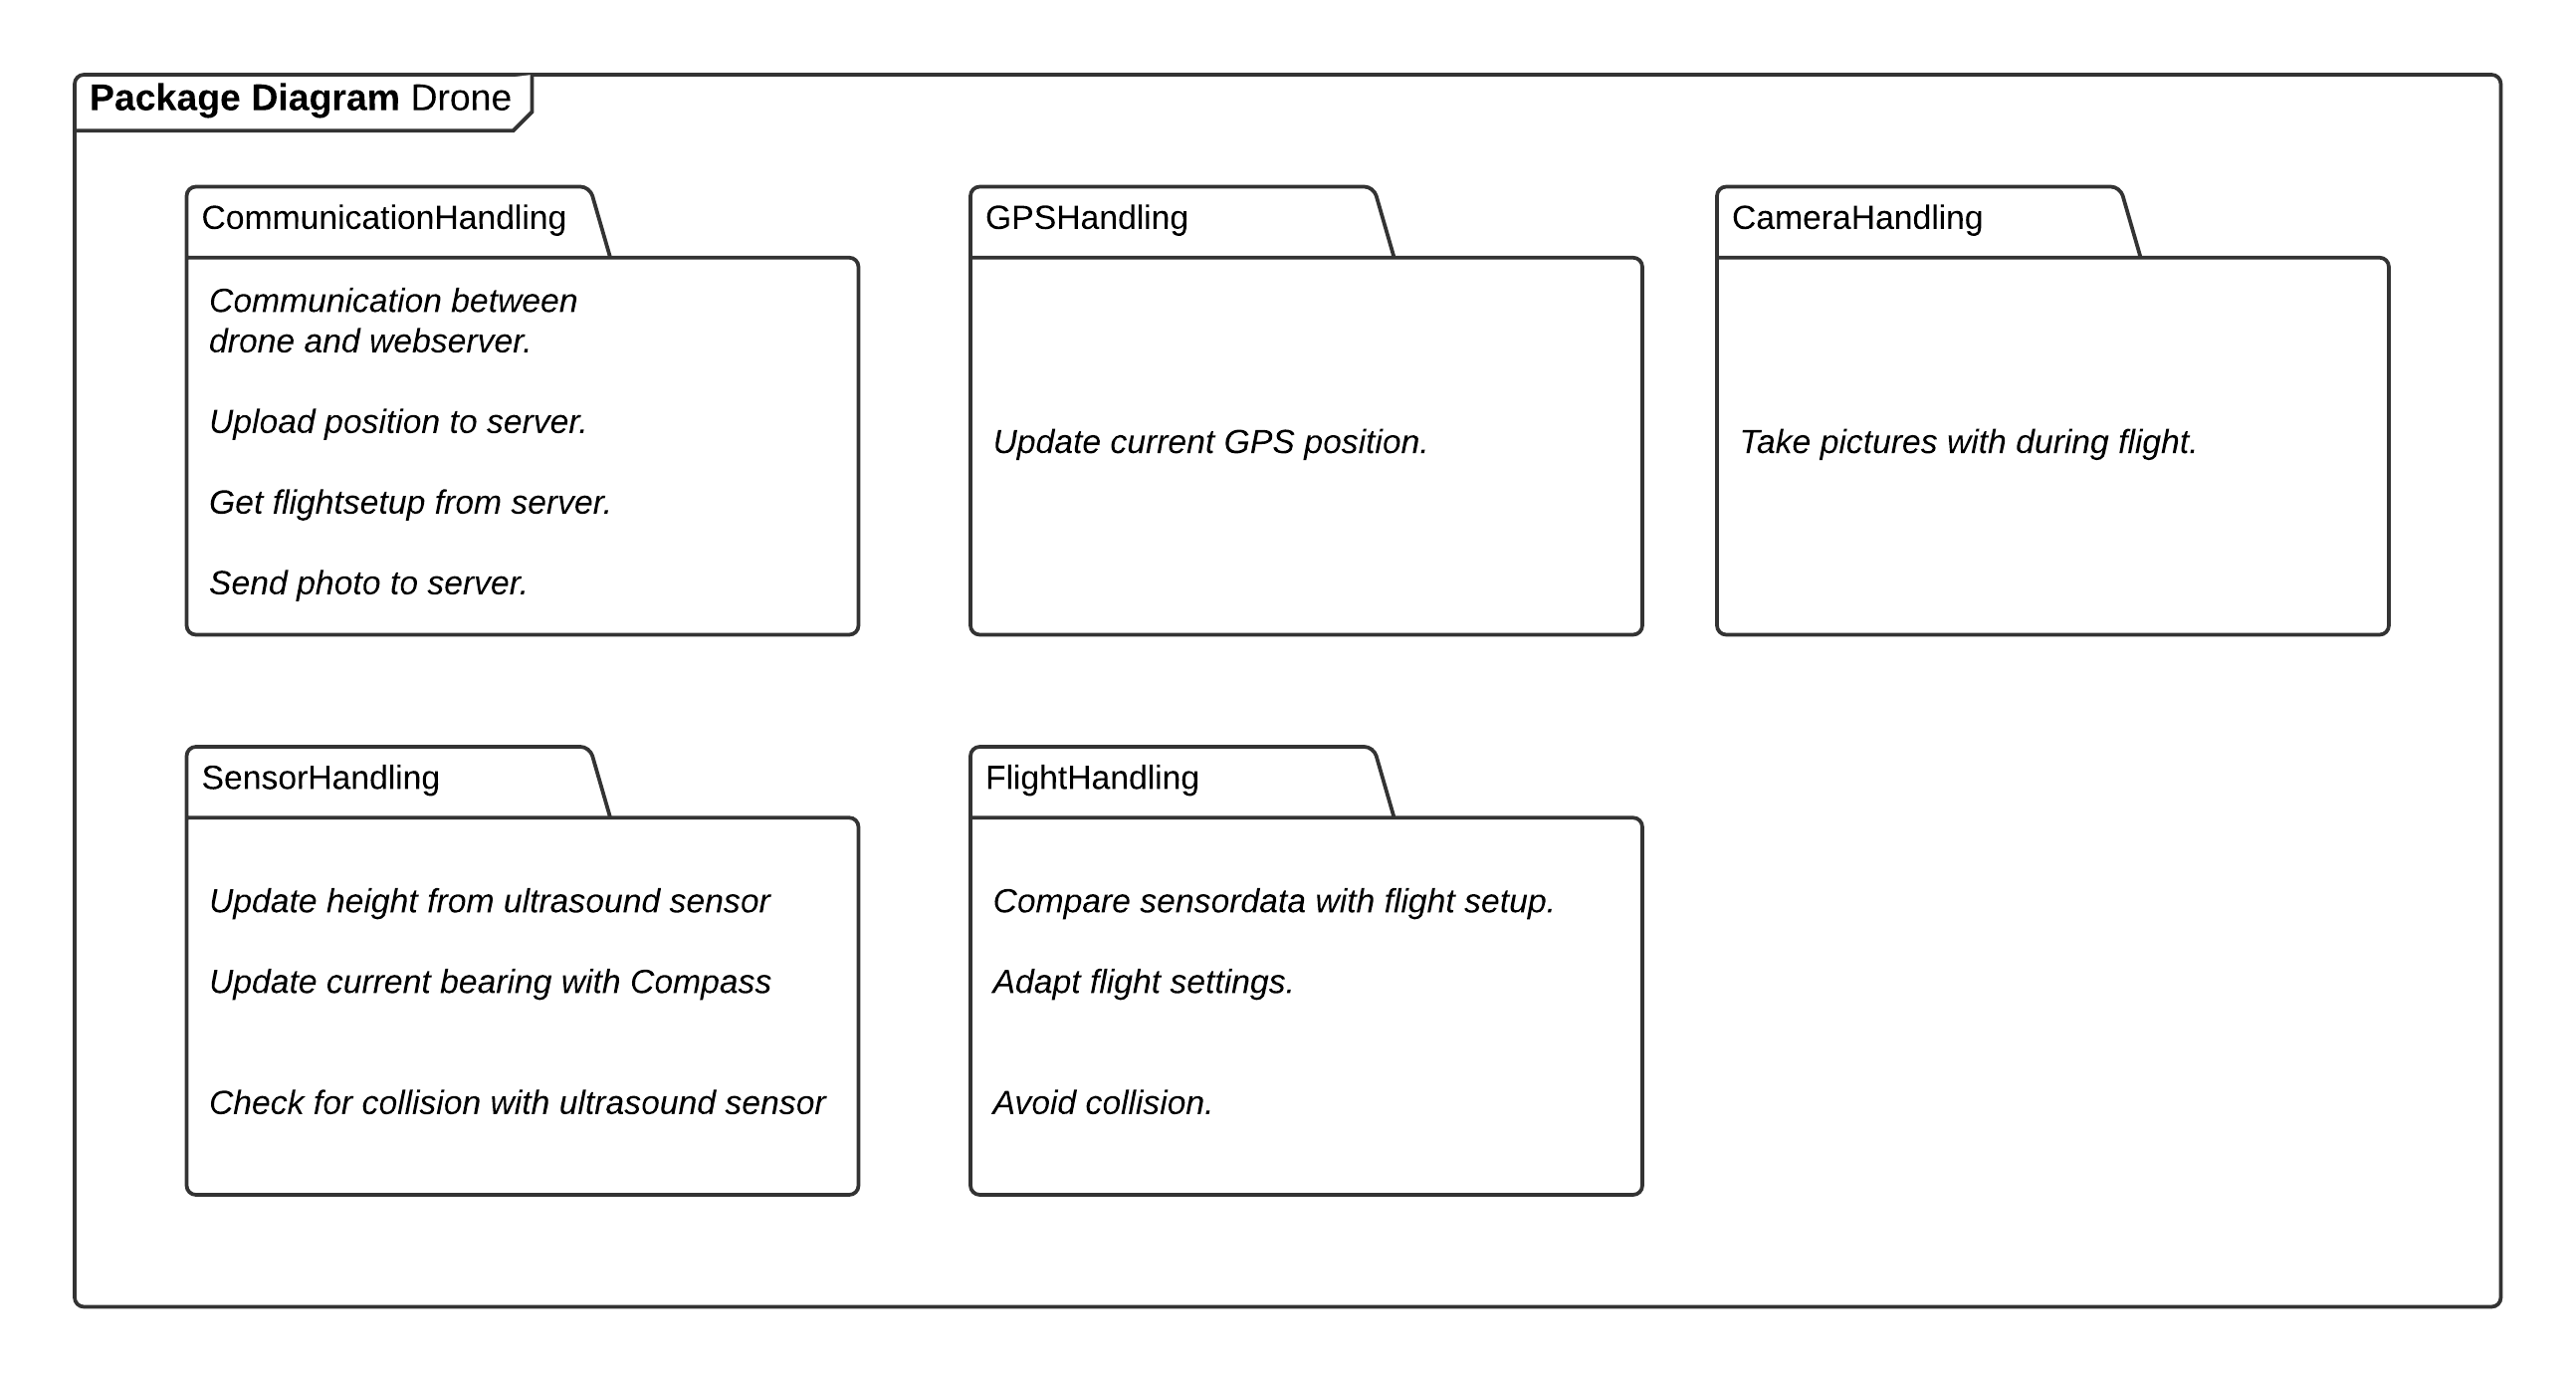
\includegraphics[width=0.85\textwidth]{Billeder/Projektbeskrivelse/Packagediagram_drone}
	\vspace{-0.3cm}	
	\caption{Overordnet pakkediagram for drone}
	\label{fig:package_drone}
\end{figure}